\subsection{Publishing venues} \label{repo_analysis_venues}

The venue where a publication was published is important information that relates documents to one another regarding the topics they discuss. For example, the publishing venue of an article is a journal. Theses don't have publishing venues, as they serve another purpose (namely, evaluating the student's knowledge and ability). In this section, we discuss the publishing venue for each type of document. Given that how the venue is stored differs depending on the repository, we look at each of them separately.

Table \ref{tab:publishing_venues} shows the most common field names per publication type and repository. For example, all 3,233 articles present in depositonce have the name of the journal they were published in stored in a field called \textit{``journalTitle''}. Books in refubium often have two fields named \textit{``series''}, one for the name of the series and the other for the issue number that corresponds to the book.

The most popular venue is called ``Sonderforschungsbereich 649: Ökonomisches Risiko'' which appears on 809 publications of edoc. The second most popular venue is also a ``Sonderforschungsbereich'' of the \acrshort{hu} (which means ``research area in English'') and it appears in 583 publications. The third one is the first real publishing venue: ``PLoS ONE'', with 533 publications.

On average, venues appear on 4.2 publications. There are 4,418 venues present across all three repositories, 2,867 of which (65 \%) are only assigned to one publication. From this follows that 2,867 publications (15 \%) have a venue which they don't share with any other publication. As shown in figure \ref{fig:pubs_venue_alone}, more than half of these publications belong to refubium. Furthermore, 292 publications (2 \%) don't have a venue, almost half of them belonging to depositonce. The amount of these publications that belong to each repository is illustrated in figure \ref{fig:pubs_with_no_venue}.

\begin{table}
\centering
\begin{tabular}{|c|c|c|c|c|}
\hline
\thead{Doc. type} & \thead{Repository} & \thead{\# docs} & \thead{Field name} & \thead{\# fields} \\
\hline\hline
\multirow{3}{*}{Article} & depositonce & 3233 & journalTitle & 3233 \\ \cline{2-5}
& edoc & 1904 & container-title & 1846 \\ \cline{2-5}
& refubium & 7519 & journalTitle & 3517 \\ \cline{2-5}
\hline
\multirow{3}{*}{Book part} & depositonce & 155 & bookTitle & 155 \\ \cline{2-5}
& edoc & 160 & container-title & 214 \\ \cline{2-5}
& refubium & 172 & bookTitle & 109 \\ \cline{2-5}
\hline
\multirow{3}{*}{Book} & depositonce & 91 & series & 118 \\ \cline{2-5}
& edoc & 2128 & container-title & 2076 \\ \cline{2-5}
& refubium & 1184 & series & 2211 \\ \cline{2-5}
\hline
\multirow{3}{*}{Conference Obj.} & depositonce & 465 & series & 450 \\ \cline{2-5}
& edoc & 489 & container-title & 993 \\ \cline{2-5}
& refubium & 378 & series & 0 \\ \cline{2-5}
\hline
\end{tabular}
\caption{Field names where the publishing venues are stored per document type and repository.}
\label{tab:publishing_venues}
\end{table}

\begin{figure}
  \begin{subfigure}[t]{0.45\textwidth}
    \centering
    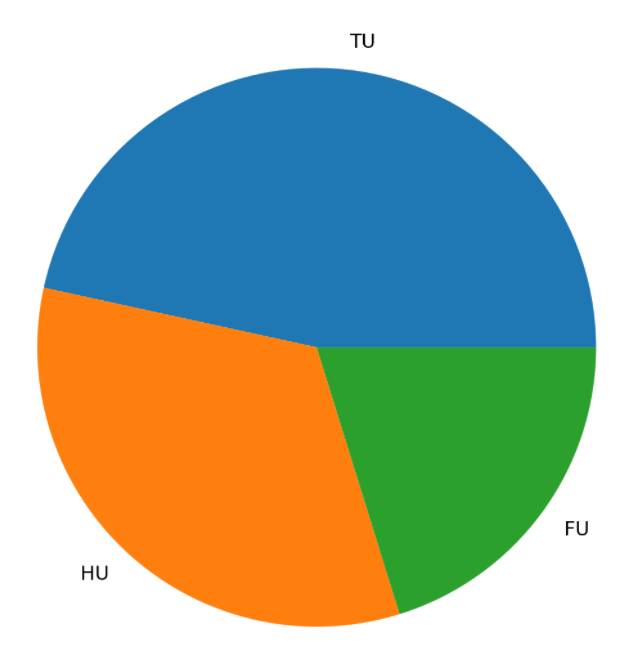
\includegraphics[width=\textwidth]{figures/repository_analysis/pubs_with_no_venue.PNG}
    \caption{Publications with no venue}
    \label{fig:pubs_with_no_venue}
  \end{subfigure}
  \hfill
  \begin{subfigure}[t]{0.41\textwidth}
    \centering
    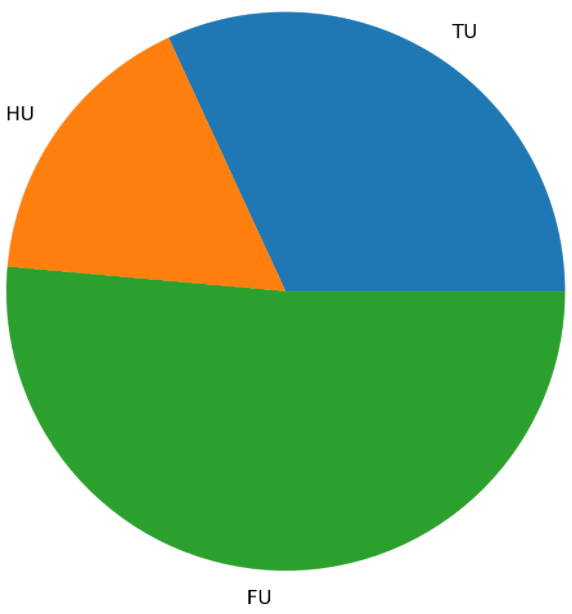
\includegraphics[width=\textwidth]{figures/repository_analysis/pubs_venue_alone.PNG}
    \caption{Publications that don't share the venue with any other publication.}
    \label{fig:pubs_venue_alone}
  \end{subfigure}
  \caption{Pie charts about the venues of the publications.}
\end{figure}